\PassOptionsToPackage{unicode=true}{hyperref} % options for packages loaded elsewhere
\PassOptionsToPackage{hyphens}{url}
\documentclass[11pt,ignorenonframetext,aspectratio=169]{beamer}
\IfFileExists{pgfpages.sty}{\usepackage{pgfpages}}{}
\setbeamertemplate{caption}[numbered]
\setbeamertemplate{caption label separator}{: }
\setbeamercolor{caption name}{fg=normal text.fg}
\beamertemplatenavigationsymbolsempty
\usepackage{lmodern}
\usepackage{amssymb,amsmath}
\usepackage{ifxetex,ifluatex}
\usepackage{fixltx2e} % provides \textsubscript
\ifnum 0\ifxetex 1\fi\ifluatex 1\fi=0 % if pdftex
  \usepackage[T1]{fontenc}
  \usepackage[utf8]{inputenc}
\else % if luatex or xelatex
  \ifxetex
    \usepackage{mathspec}
  \else
    \usepackage{fontspec}
\fi
\defaultfontfeatures{Ligatures=TeX,Scale=MatchLowercase}







\fi

  \usetheme[]{metropolis}






% use upquote if available, for straight quotes in verbatim environments
\IfFileExists{upquote.sty}{\usepackage{upquote}}{}
% use microtype if available
\IfFileExists{microtype.sty}{%
  \usepackage{microtype}
  \UseMicrotypeSet[protrusion]{basicmath} % disable protrusion for tt fonts
}{}


\newif\ifbibliography
  \usepackage[]{biblatex}
      \addbibresource{./../bibliographies.bib}
  

\hypersetup{
      pdftitle={Introduction to plant breeding},
        pdfauthor={Deependra Dhakal},
          pdfborder={0 0 0},
    breaklinks=true}
%\urlstyle{same}  % Use monospace font for urls







% Prevent slide breaks in the middle of a paragraph:
\widowpenalties 1 10000
\raggedbottom

  \AtBeginPart{
    \let\insertpartnumber\relax
    \let\partname\relax
    \frame{\partpage}
  }
  \AtBeginSection{
    \ifbibliography
    \else
      \let\insertsectionnumber\relax
      \let\sectionname\relax
      \frame{\sectionpage}
    \fi
  }
  \AtBeginSubsection{
    \let\insertsubsectionnumber\relax
    \let\subsectionname\relax
    \frame{\subsectionpage}
  }



\setlength{\parindent}{0pt}
\setlength{\parskip}{6pt plus 2pt minus 1pt}
\setlength{\emergencystretch}{3em}  % prevent overfull lines
\providecommand{\tightlist}{%
  \setlength{\itemsep}{0pt}\setlength{\parskip}{0pt}}

  \setcounter{secnumdepth}{0}


  \usepackage{setspace}
  \usepackage{wasysym}
  % \usepackage{fontenc}
  \usepackage{booktabs,siunitx}
  \usepackage{longtable}
  \usepackage{array}
  \usepackage{multirow}
  \usepackage{wrapfig}
  \usepackage{float}
  \usepackage{colortbl}
  \usepackage{pdflscape}
  \usepackage{tabu}
  \usepackage{threeparttable}
  \usepackage{threeparttablex}
  \usepackage[normalem]{ulem}
  \usepackage{makecell}
  \usepackage{xcolor}
  \usepackage{tikz} % required for image opacity change
  \usepackage[absolute,overlay]{textpos} % for text formatting
  \usepackage[skip=0.333\baselineskip]{caption}
  % \usepackage{newtxtext,newtxmath}% better than txfonts   
  \usepackage[english]{babel}
  \usepackage{pgfpages}

  \sisetup{per-mode=symbol}

  % % Added by CII
  % \usepackage[format=hang,labelfont=bf,margin=0.5cm,justification=centering]{caption}
  % \captionsetup{font=small,width=0.9\linewidth,labelfont=small,textfont={small}}
  % % End of CII addition

  % \usepackage{subcaption}
  % \newcommand{\subfloat}[2][need a sub-caption]{\subcaptionbox{#1}{#2}}

  \captionsetup[sub]{font=footnotesize,labelfont=footnotesize,textfont=footnotesize}
  % \captionsetup[subfigure]{font=small,labelfont=small,textfont=small}
  % \captionsetup[subfloat]{font=scriptsize,labelfont=scriptsize,textfont=scriptsize}

  % this font option is amenable for beamer, although these are global settings
  \setbeamerfont{caption}{size=\tiny}
  % \setbeamerfont{subcaption}{size=\tiny} % this does not chage subfloat fonts
  % \setbeamerfont{subfloat}{size=\tiny} % this does not change subfloat fonts
   
   % use single line spacing ?
  \singlespacing

  % use cslreferences environment
  % this is revised as of Oct, 2022 (https://stackoverflow.com/questions/59193797/pandocs-environment-cslreferences-undefined-when-knitting-rmarkdown-to-pdf-in-r)
  \newlength{\cslhangindent}
  \setlength{\cslhangindent}{1.5em}
  \newenvironment{CSLReferences}%
    {\setlength{\parindent}{0pt}%
    \everypar{\setlength{\hangindent}{\cslhangindent}}\ignorespaces}%
    {\par}


  \newcommand{\bcolumns}{\begin{columns}[T, onlytextwidth]}
  \newcommand{\ecolumns}{\end{columns}}

  \newcommand{\bdescription}{\begin{description}}
  \newcommand{\edescription}{\end{description}}

  \newcommand{\bitemize}{\begin{itemize}}
  \newcommand{\eitemize}{\end{itemize}}
  % notes will be showed

  % \setbeamertemplate{note page}{\insertnote} % a plain style
  \setbeameroption{show notes}

  % 
  % \usepackage{etoolbox}
  % 
  % % use different background canvas
  % \defbeamertemplate{background canvas}{ddefault}{%
  %   \includegraphics[width=\paperwidth,height=\paperheight]{}
  % }
  % \defbeamertemplate{background canvas}{standout}{%
  %   \includegraphics[width=\paperwidth,height=\paperheight]{}
  % }
  % 
  % \BeforeBeginEnvironment{frame}{%
  %   \setbeamertemplate{background canvas}[ddefault]%
  % }
  % 
  % \makeatletter
  % \define@key{beamerframe}{standout}[true]{%
  %   \setbeamertemplate{background canvas}[standout]%
  % }
  % \makeatother

  % % use different frame headline styles
  % \defbeamertemplate{headline}{mydefault}{%
  %   \rule{.5\paperwidth}{14mm}%
  % }
  % \defbeamertemplate{headline}{rightslide}{%
  %   \emph{\hfill\rule{.5\paperwidth}{14mm}}%
  % }
  % 
  % \BeforeBeginEnvironment{frame}{%
  %   \setbeamertemplate{headline}[mydefault]%
  % }
  % 
  % \makeatletter
  % \define@key{beamerframe}{rightslide}[true]{%
  %   \setbeamertemplate{headline}[rightslide]%
  % }
  % \makeatother
  \setbeamercolor{block body alerted}{bg=alerted text.fg!10}
  \setbeamercolor{block title alerted}{bg=alerted text.fg!20}
  \setbeamercolor{block body}{bg=blue!10}
  \setbeamercolor{block title}{bg=blue!30}
  \setbeamercolor{block body example}{bg=green!10}
  \setbeamercolor{block title example}{bg=green!20}

  \title[]{Introduction to plant breeding}


  \author[
        Deependra Dhakal
    ]{Deependra Dhakal}

  \institute[
    ]{
    Assistant Professor\\
Agriculture and Forestry University\\
\textit{ddhakal.rookie@gmail.com}\\
\url{https://rookie.rbind.io}
    }

\date[
      
  ]{
    }


\begin{document}

% Hide progress bar and footline on titlepage
  \begin{frame}[plain]
  \titlepage
  \end{frame}



\hypertarget{introduction}{%
\section{Introduction}\label{introduction}}

\begin{frame}{}
\protect\hypertarget{section}{}
\begin{center}\includegraphics[width=0.8\linewidth]{./images/x_men_mutants} \end{center}
\end{frame}

\begin{frame}{What experts say\ldots{}}
\protect\hypertarget{what-experts-say}{}
\bcolumns
\column{0.65\textwidth}

\begin{quote}
\small
"For more than half a century, I have worked with the production of more and better wheat for feeding the hungry world, but wheat is merely a catalyst, a part of the picture. I am interested in the total development of human beings. Only by attacking the whole problem can we raise the standard of living for all people, in all communities, so that they will be able to live decent lives. This is something we want for all people on this planet".
\end{quote}
\hfill\raggedright{\footnotesize -- Norman E. Borlaug (March 25,1914 - September 12, 2009)}

\column{0.35\textwidth}

\begin{figure}
\includegraphics[width=0.95\linewidth]{./images/borlaug_wheat_crossing_block} \caption{Dr. Borlaug working in a wheat crossing block}\label{fig:borlaug}
\end{figure}

\ecolumns
\end{frame}

\begin{frame}{}
\protect\hypertarget{section-1}{}
\begin{columns}[T,c,onlytextwidth]
\column{0.4\textwidth}

\begin{quote}
\vfill
"The greatest service which can be rendered any country is to add a useful plant to its culture; especially a bread grain"
\end{quote}
\hfill\raggedright{\footnotesize -- Thomas Jefferson}

\column{0.6\textwidth}

\begin{figure}
\includegraphics[width=0.75\linewidth]{./images/Triticum3} \caption{Modern wheat genotype under test in cool temperate region (UK)}\label{fig:modern-triticum-uk}
\end{figure}

\end{columns}
\end{frame}

\begin{frame}{Background (Overview)}
\protect\hypertarget{background-overview}{}
\begin{itemize}
\tightlist
\item
  There are over a quarter of a million plant species of which
  approximately 5000 are cultivated. But, only a 100 can be considered
  as important crops.
\item
  Ancestors of most of the modern crops (Used either in food chain or in
  industrial chain solely) have different appearance and even forms than
  what is seen today.
\item
  Plant breeding has a commercial history of 2/3 century at least.
\item
  By 19th century's end, artificial crossing, bulk and pedigree methods
  and alternative progeny testing schems were already used
\end{itemize}
\end{frame}

\begin{frame}{}
\protect\hypertarget{section-2}{}
\begin{itemize}
\tightlist
\item
  After rediscovery of Mendel's law and developments in genetics plant
  breeding has evolved rapidly
\item
  In the period deemed green revolution, genetic contribution to yield
  gains was of secondary importance (Why?)
\item
  Rising consciousness of environmental stewardship underlines greater
  role of plant breeding

  \begin{itemize}
  \tightlist
  \item
    Optimum environments
  \item
    Marginal environments
  \item
    Economic value of resources
  \end{itemize}
\item
  Extermely wide and cross cutting topic nowadays!
\item
  Plant breeding has answered many fundamental genetic questions and
  posed new ones too.
\end{itemize}
\end{frame}

\hypertarget{concept}{%
\section{Concept}\label{concept}}

\begin{frame}{}
\protect\hypertarget{section-3}{}
\begin{columns}[T,onlytextwidth]
\begin{column}{0.5\textwidth}
"Breeder's eye" viewpoint of Plant Breeding: 
\begin{itemize}
\item Plant breeding is an applied science and an art 
\item Early plant breeders depended primarily on intuition, skill, and judgement in their work.
\item Plant breeding was practiced first when people learned to look for superior plants to harvest for seed; thus selection became the earliest method of plant breeding. However few people may have had conscious efforts in so-doing.
\end{itemize}
\end{column}
\begin{column}{0.5\textwidth}  %%<--- here
Scientific viewpoint of Plant Breeding: 
\begin{itemize}
\item "Breeding" is about a more active process of crossing different strains of plant for particular results.
\item Plant evolution directed by man (N.I. Vavilov)
\item Process of generating and utilizing variability
\item "Selection" is about picking the best from each generation
\end{itemize}
\end{column}
\end{columns}
\end{frame}

\begin{frame}{}
\protect\hypertarget{section-4}{}
\begin{itemize}
\item
  As human knowledge about plants increased, people were able to select
  more intelligently.
\item
  With the discovery of sex in plants, hybridization was added to
  breeding techniques.
\item
  Although hybridization was practiced before the time of Mendel, its
  significance in inheritance was not clearly understood.
\item
  Mendel's experiments provided a basis for understanding the mechanism
  of heredity and how it may be manipulated in the development of
  improved varieties.
\item
  A more precise explanation of the heredity mechanism has become
  possible in recent years with advances in biochemical genetics.
\item
  Now, plant breeding is more about making precise crossess and accurate
  prediction
\end{itemize}

\[\Large \Delta{G}=\frac{Ih^2 \sigma}{I}\]
\end{frame}

\hypertarget{definition}{%
\section{Definition}\label{definition}}

\begin{frame}{}
\protect\hypertarget{section-5}{}
\bcolumns
\column{0.65\textwidth}

\begin{block}{Plant breeding}
The art and the science of changing and improving the heredity of plants
\end{block}

\begin{itemize}
\tightlist
\item
  Breeding is about manipulating plant attributes, structure and
  composition, to make them more useful to humans.
\item
  Plant breeding is essentially an election made by man of the best
  plants within a variable population as a potential cultivar.
\item
  In other words plant breeding is a `selection' made possible by the
  existence of `variability'.
\end{itemize}

\column{0.35\textwidth}

\textbf{How do you define art?}

\includegraphics[width=0.45\linewidth]{images/life-of-an-artist-funny-comics-9}

\includegraphics[width=0.65\linewidth]{images/art-negative-space-design-art-illustration}

\ecolumns
\end{frame}

\hypertarget{history}{%
\section{History}\label{history}}

\begin{frame}{History (Overview)}
\protect\hypertarget{history-overview}{}
\begin{itemize}
\tightlist
\item
  Broadly, two distinct stages in plant breeding could be characterized

  \begin{itemize}
  \tightlist
  \item
    Domestication of the first crops to the birth of Mendelian genetics
  \item
    Acceptance of Medelian genetics to post-mendel era
  \end{itemize}
\item
  The work of Gregor Mendel and further advances in science that
  followed his discoveries established that plant traits are controlled
  by hereditary factors or genes that consist of DNA (deoxyribose
  nucleic acid, the hereditary material).
\end{itemize}
\end{frame}

\begin{frame}{History (Pre-mendel era)}
\protect\hypertarget{history-pre-mendel-era}{}
\begin{itemize}
\tightlist
\item
  Plant breeding started with sedentary agriculture and the
  domestication of the first agricultural plants, the cereals, which
  were chosen by early man.
\item
  A family of French seed growers, the Vilmorins, established in 1727
  the first company devoted to plant breeding and the production of new
  varieties.
\item
  The sexuality of plants was described by Caesalpinus in 1583 and in
  1696 Camerarius published an essay entitled `De sexo plantarum', but
  it was Kolreuter, a German botanist who was the first to exploit this
  knowledge in the production of the first artificial plant hybrids in
  Nicotiana.
\end{itemize}
\end{frame}

\begin{frame}{History (Post-mendel era)}
\protect\hypertarget{history-post-mendel-era}{}
\begin{itemize}
\tightlist
\item
  After the rediscovery of the work of Mendel in 1900 it was some six
  years before Bateson, who coined the name `genetics' for the new
  science, realized that this new discipline could give a scientific
  basis and new openings to plant breeding methods.
\item
  Genetics has given to breeding a better knowledge of the processes
  involved in the mechanisms of variability and the necessary
  information for regulating and increasing such variability.
\end{itemize}
\end{frame}

\begin{frame}{History (Domestication and evolution)}
\protect\hypertarget{history-domestication-and-evolution}{}
\begin{figure}
\includegraphics[width=0.6\textwidth, keepaspectratio,height=0.38\textheight]{./images/rye_crop} \caption{Image of ancestor of wheat \textit{Secale cereale}}\label{fig:secale-cereale}
\end{figure}

\begin{figure}
\includegraphics[width=0.6\textwidth, keepaspectratio,height=0.38\textheight]{./images/wheat_borlaug-100} \caption{Modern wheat \textit{Triticum aestivum}}\label{fig:modern-wheat}
\end{figure}
\end{frame}

\begin{frame}{}
\protect\hypertarget{section-6}{}
\begin{figure}
\includegraphics[width=0.6\textwidth, keepaspectratio,height=0.45\textheight]{./images/rose_prickly_or_common} \caption{rose ancestor (Wild rose)}\label{fig:rose-wild}
\end{figure}

\begin{figure}
\includegraphics[width=0.6\textwidth, keepaspectratio,height=0.45\textheight]{./images/rose-modern} \caption{Rose modern}\label{fig:rose-modern}
\end{figure}
\end{frame}

\begin{frame}{}
\protect\hypertarget{section-7}{}
\begin{figure}
\includegraphics[width=0.45\linewidth,height=0.4\textheight]{./images/Tomato_galapagos_Solanum-cheesmanii} \caption{Wild tomato (Lycopersicum cheesmanii); Unique and rare, wild, small cherry tomato from the rocky, lava flow areas of Ecuador's famed Galapagos Islands. These cherry shaped, yellowish-orange fruited tomatoes are flavorful and have lemon scented foliage. They enjoy heat and tolerate drought. Similar to cultivated tomatoes in flavor but with more disease and insect tolerance, as well as salt water tolerance. Plants typically vine, are very productive, and easy to grow.}\label{fig:tomato-wild}
\end{figure}

\begin{figure}
\includegraphics[width=0.6\textwidth, keepaspectratio,height=0.4\textheight]{./images/modified_tomatoes} \caption{Modern tomato (Lycopersicum esculentum)}\label{fig:tomato-modern}
\end{figure}
\end{frame}

\begin{frame}{}
\protect\hypertarget{section-8}{}
\begin{figure}
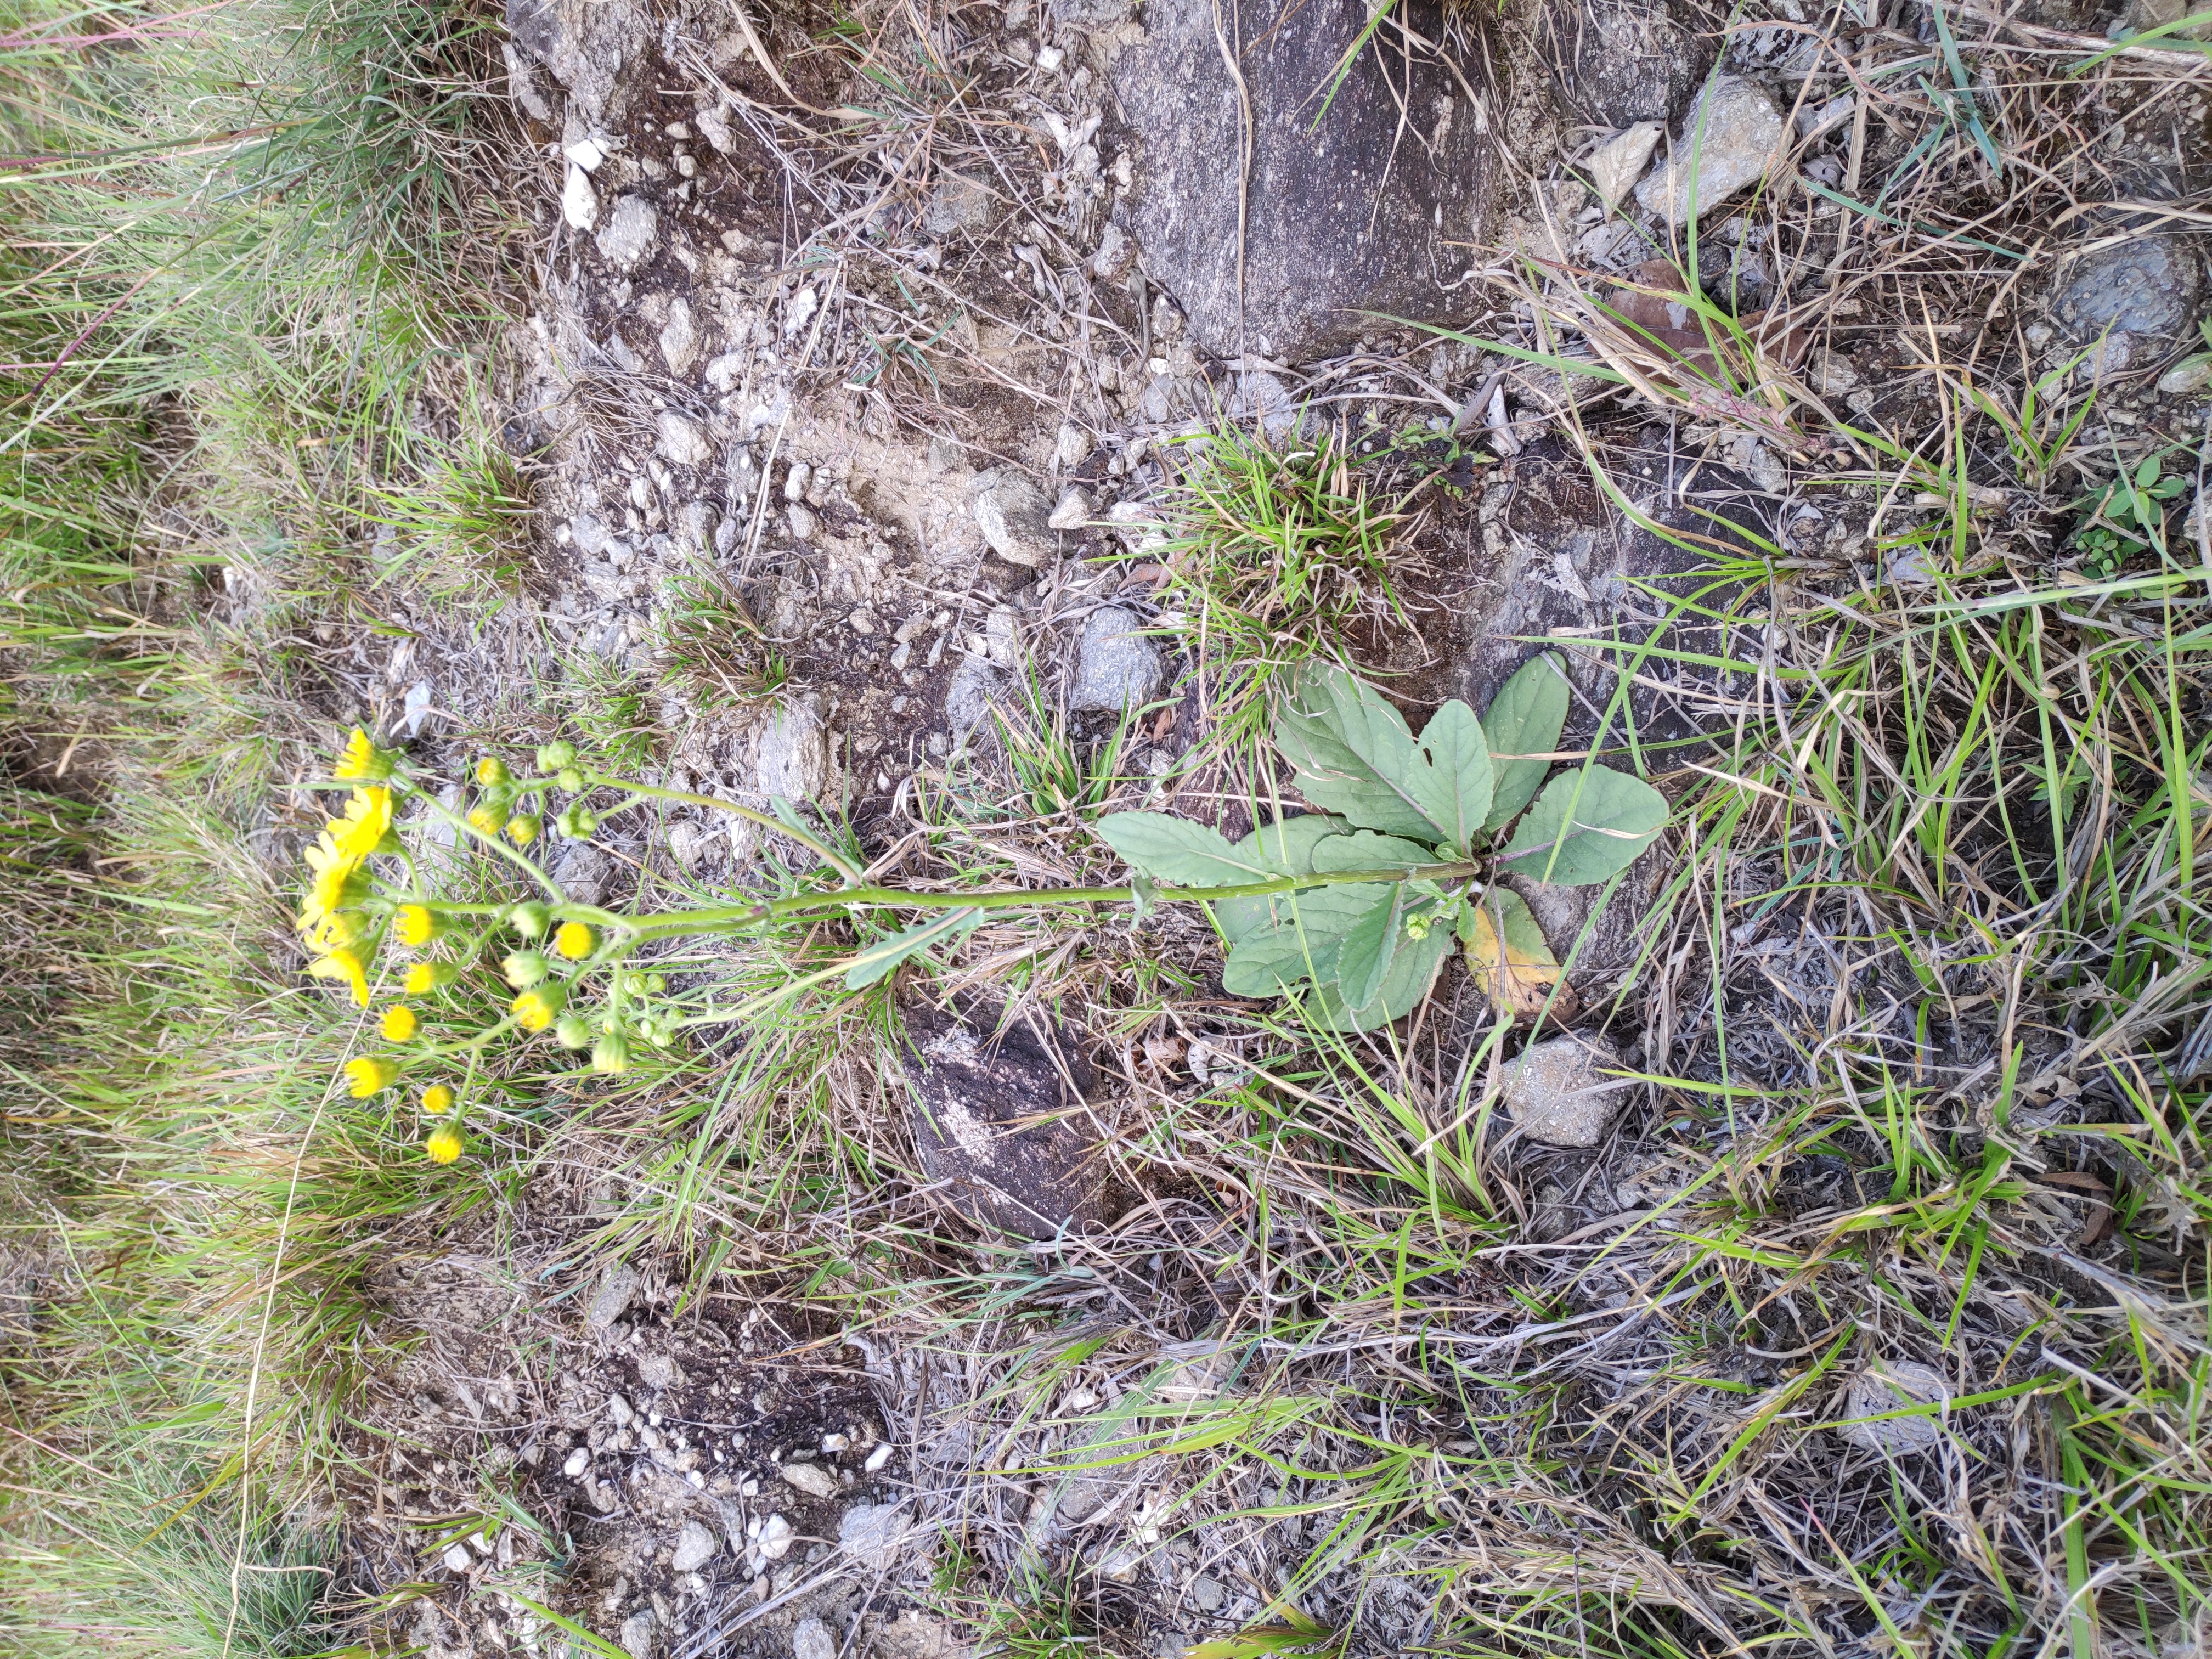
\includegraphics[width=0.6\textwidth, keepaspectratio,height=0.45\textheight]{./images/brassica_arabidopsis} \caption{Arabidopsis spp.}\label{fig:wild-brassica}
\end{figure}

\begin{figure}
\includegraphics[width=0.6\textwidth, keepaspectratio,height=0.45\textheight]{./images/Ornamental_cabbage} \caption{Modern day cauliflower}\label{fig:modern-brassica}
\end{figure}
\end{frame}

\begin{frame}{}
\protect\hypertarget{section-9}{}
\begin{figure}
\includegraphics[width=0.6\textwidth, keepaspectratio,height=0.45\textheight]{./images/Teosinte} \caption{Wild progenitor of modern day maize -- Teosinte}\label{fig:maize-ancestor-teosinte}
\end{figure}

\begin{figure}
\includegraphics[width=0.6\textwidth, keepaspectratio,height=0.45\textheight]{./images/Teosinte_maize} \caption{Modern day maize (Zea mays)}\label{fig:maize-modern}
\end{figure}
\end{frame}

\begin{frame}{History (Interesting facts)}
\protect\hypertarget{history-interesting-facts}{}
\bcolumns
\column{0.65\textwidth}
\small

\begin{itemize}
\tightlist
\item
  Historically, good seed from high-yielding plants were stored in woven
  baskets and bartered for metal tools or cloth.
\item
  Nowadays test tubes and computers have replaced the baskets, and huge
  research budgets have replaced the barter.
\item
  Luther Burbank is the last great prescientific plant breeder.
\item
  Burbank admired Darwin but not Mendel
\item
  Remarkably strong start in plant breeding was made by Soviet
  Communists in twentieth century. But dissapointingly, intrigue and
  ideology ensured that Mendelian genetics was discarded.
\item
  For detailed history refer to Principles of Plant Genetics and
  Breeding \autocite{acquaah2009principles}, Chapter 2 (Page 22-39).
\item
  For detailed history of Genetics refer to
  \textcite{griffiths2015introduction} .
\end{itemize}

\column{0.35\textwidth}
\begin{quote}
\scriptsize
"Charles Darwin's writing in the nineteenth century first formulated the idea of evolution, the idea that plants and animals are in constant competition, which results in the fittest or the best adapted surviving and passing on their genes to the next generation, those less well-adapted dying or failing to reproduce and so not passing on their genetic code. Life, then, is a constant winnowing and sifting of genetic material." 
\end{quote}

\ecolumns
\end{frame}

\begin{frame}{History (Timeline)}
\protect\hypertarget{history-timeline}{}
\begin{table}

\caption{\label{tab:history-table1}History of genetics}
\centering
\fontsize{8}{10}\selectfont
\begin{tabular}[t]{l>{\raggedright\arraybackslash}p{40em}}
\toprule
Year & Event\\
\midrule
\cellcolor{gray!6}{1865} & \cellcolor{gray!6}{Gregor Mendel showed that traits are controlled by discrete factors now known as genes.}\\
1869 & Friedrich Miescher isolated DNA from the nuclei of white blood cells.\\
\cellcolor{gray!6}{1903} & \cellcolor{gray!6}{Walter Sutton and Theodor Boveri hypothesized that chromosomes are the hereditary elements.}\\
1905 & William Bateson introduced the term “genetics” for the study of inheritance.\\
\cellcolor{gray!6}{1908} & \cellcolor{gray!6}{G. H. Hardy and Wilhelm Weinberg proposed the Hardy–Weinberg law, the foundation for population genetics}\\
\addlinespace
1910 & Thomas H. Morgan demonstrated that genes are located on chromosomes.\\
\cellcolor{gray!6}{1913} & \cellcolor{gray!6}{Alfred Sturtevant made a genetic linkage map of the Drosophila X chromosome, the first genetic map.}\\
1918 & Ronald Fisher proposed that multiple Mendelian factors can explain continuous variation for traits, founding the field of quantitative genetics.\\
\cellcolor{gray!6}{1931} & \cellcolor{gray!6}{Harriet Creighton and Barbara McClintock showed that crossing over is the cause of recombination.}\\
1941 & Edward Tatum and George Beadle proposed the one-gene—one-polypeptide hypothesis.\\
\bottomrule
\end{tabular}
\end{table}
\end{frame}

\begin{frame}{}
\protect\hypertarget{section-10}{}
\begin{table}

\caption{\label{tab:history-table2}History of genetics...}
\centering
\fontsize{8}{10}\selectfont
\begin{tabular}[t]{l>{\raggedright\arraybackslash}p{40em}}
\toprule
Year & Event\\
\midrule
\cellcolor{gray!6}{1944} & \cellcolor{gray!6}{Oswald Avery, Colin MacLeod, and Maclyn McCarty provided compelling evidence that DNA is the genetic material in bacterial cells.}\\
1946 & Joshua Lederberg and Edward Tatum discovered bacterial conjugation.\\
\cellcolor{gray!6}{1948} & \cellcolor{gray!6}{Barbara McClintock discovered mobile elements (transposons) that move from one place to another in the genome.}\\
1950 & Erwin Chargaff showed DNA composition follows some simple rules for the relative amounts of A, C, G, and T.\\
\cellcolor{gray!6}{1952} & \cellcolor{gray!6}{Alfred Hershey and Martha Chase proved that DNA is the molecule that encodes genetic information.}\\
\addlinespace
1953 & James Watson and Francis Crick determined that DNA forms a double helix.\\
\cellcolor{gray!6}{1958} & \cellcolor{gray!6}{Matthew Meselson and Franklin Stahl demonstrated the semiconservative nature of DNA replication.}\\
1958 & Jérôme Lejeune discovered that Down syndrome resulted from an extra copy of the 21st chromosome.\\
\cellcolor{gray!6}{1961} & \cellcolor{gray!6}{François Jacob and Jacques Monod proposed that enzyme levels in cells are controlled by feedback mechanisms.}\\
1961-1967 & Marshall Nirenberg, Har Gobind Khorana, Sydney Brenner, and Francis Crick "cracked" the genetic code.\\
\bottomrule
\end{tabular}
\end{table}
\end{frame}

\begin{frame}{}
\protect\hypertarget{section-11}{}
\begin{table}

\caption{\label{tab:history-table3}History of genetics...}
\centering
\fontsize{8}{10}\selectfont
\begin{tabular}[t]{l>{\raggedright\arraybackslash}p{40em}}
\toprule
Year & Event\\
\midrule
\cellcolor{gray!6}{1968} & \cellcolor{gray!6}{Motoo Kimura proposed the neutral theory of molecular evolution.}\\
1977 & Fred Sanger, Walter Gilbert, and Allan Maxam invented methods for determining the nucleotide sequences of DNA molecules.\\
\cellcolor{gray!6}{1980} & \cellcolor{gray!6}{Christiane Nüsslein-Volhard and Eric F. Wieschaus defined the complex of genes that regulate body plan development in Drosophila.}\\
1989 & Francis Collins and Lap-Chee Tsui discovered the gene causing cystic fibrosis.\\
\cellcolor{gray!6}{1993} & \cellcolor{gray!6}{Victor Ambrose and colleagues described the first microRNA.}\\
\addlinespace
1995 & First genome sequence of a living organism (Haemophilus influenzae) published.\\
\cellcolor{gray!6}{1996} & \cellcolor{gray!6}{First genome sequence of a eukaryote (Saccharomyces cerevisiae) published.}\\
1998 & First genome sequence of an animal (Caenorhabditis elegans) published.\\
\cellcolor{gray!6}{2000} & \cellcolor{gray!6}{First genome sequence of a plant (Arabidopsis thaliana) published.}\\
2001 & The sequence of the human genome first published.\\
\addlinespace
\cellcolor{gray!6}{2006} & \cellcolor{gray!6}{Andrew Fire and Craig Mello win the Nobel prize for their discovery of gene silencing by double-stranded RNA.}\\
2012 & John Gurdon and Shinya Yamanaka win the Nobel prize for their discovery that just four regulatory genes can convert adult cells into stem cells.\\
\bottomrule
\end{tabular}
\end{table}
\end{frame}

\begin{frame}{}
\protect\hypertarget{section-12}{}
\begin{figure}
\includegraphics[width=0.4\linewidth,height=0.7\textwidth, keepaspectratio]{./images/plant_breeding_history} \caption{History of plant breeding Rolf H. J. Schlegel, 2018}\label{fig:plb-history-book}
\end{figure}
\end{frame}

\hypertarget{objectives}{%
\section{Objectives}\label{objectives}}

\begin{frame}{}
\protect\hypertarget{section-13}{}
\small

\begin{itemize}
\tightlist
\item
  Before initiating a breeding project, clear breeding objectives are
  defined based on factors such as producer needs, consumer preferences
  and needs, and environmental impact.
\end{itemize}

\textbf{Broad objectives}

\begin{itemize}
\tightlist
\item
  Feed the growing population
\item
  Maximize resource and energy use efficiency
\item
  Fasten return on investment
\item
  Introgress desired modification in crop species
\end{itemize}
\end{frame}

\begin{frame}{Specifically, in crop improvement,}
\protect\hypertarget{specifically-in-crop-improvement}{}
\small

\begin{itemize}
\tightlist
\item
  Increasing the potential productivity of a plant by modifying its
  morphological characteristics such as:

  \begin{itemize}
  \footnotesize
  \item The number of kernels per ear in a cereal
  \item The weight of individual seeds within the pod of a pulse
  \end{itemize}
\item
  Modifying physiological traits such as:

  \begin{itemize}
  \footnotesize
  \item harvest index, 
  \item utilization of nutrients,
  \item tolerance to stress.
  \end{itemize}
\item
  Quality and nutritive value are now of increasing importance,
  particularly in association with improved efficiency of production.
\item
  Modern agriculture is highly mechanized and for this reason some
  breeding programmes include objectives to make the crop more amenable
  to mechanical handling.

  \begin{itemize}
  \footnotesize
  \item Development of monogerm beets for mechanical sowing thus eliminating the need for thinning, or the introduction of 'jointless' tomatoes for mechanical harvesting. 
  \item Use of some agrochemicals is often coupled with the need for specific crop characteristics e.g. herbicide resistance.
  \end{itemize}
\end{itemize}
\end{frame}

\begin{frame}{Activities}
\protect\hypertarget{activities}{}
\begin{figure}
\includegraphics[width=0.7\textwidth,keepaspectratio,height=0.6\textheight]{./images/interdisciplinary_science} \caption{Inter-desciplinary linkage of plant breeding}\label{fig:plb-disciplines}
\end{figure}
\end{frame}

\begin{frame}{Inter-disciplinary linkage of plant breeding
\autocite{poehlman1987breeding}}
\protect\hypertarget{inter-disciplinary-linkage-of-plant-breeding-poehlman1987breeding}{}
\small

\begin{itemize}
\tightlist
\item
  Botany: Plant breeders should be accomplished botanists in order to
  understand the taxonomy, anatomy, morphology, and reproduction of the
  plants with which they work.
\item
  Genetics and Cytogenetics: The plant breeder needs a thorough
  understanding of the mechanism of heredity in plants since modern
  plant-breeding methods are based on a knowledge of genetic principles
  and chromosome behavior. This knowledge is being extended to the
  molecular level with advances in biochemical genetics.
\item
  Plant Physiology: Variety adaptation is determined by the response of
  plants to their environment, which includes the effects of heat, cold,
  drought, and soil nutrient response. The plant breeder strives to make
  inherent modifications of physiological processes that will enable the
  plant to function more efficiently.
\item
  Plant Pathology: Plant disease reduces crop yields. Host resistance is
  an important means of combating many plant diseases. Evaluation of the
  response ofthe plant genotype to infection by the pathogen is an
  essential part of breeding for host plant resistance.
\item
  Entomology: Biological control of insect populations by breeding for
  insect resistance is an important way of reducing insect damage in
  crop plants.
\end{itemize}
\end{frame}

\begin{frame}{}
\protect\hypertarget{section-14}{}
\small

\begin{itemize}
\tightlist
\item
  Plant Biochemistry: Inherent improvements in the nutritive value of a
  crop variety are given attention by the plant breeder. Suitability for
  industrial utilization often determines the market demand for a
  particular variety of a crop. This includes such characteristics as
  the milling and baking qualities of a wheat variety, the cooking and
  eating qualities of a rice variety, or the fiber qualities of a cotton
  variety. Biochemical genetics is contributing toward a better
  understanding of the structure and function of the gene.
\item
  Statistics: The plant breeder compares the performance of many
  genetically different strains. Sound field plot techniques and
  suitable methods for statistical analyses of data are necessary to
  obtain reliable results and to interpret the results correctly. The
  application of statistical procedures has provided for a better
  understanding of the inheritance of quantitative characteristics and
  for predicting the possible genetic advance that may be obtained with
  particular systems of mating.
\item
  Agronomy: In addition to all of these, the breeder of field crops
  should be a sound agronomist. Plant breeders should know crops and
  their production. They should understand what the farmer wants and
  needs in the way of new varieties. Only then will they be able to
  evaluate critically the breeding materials available to them, plan an
  efficient breeding program, and direct their breeding efforts toward
  the agronomically important objectives.
\end{itemize}
\end{frame}

\hypertarget{steps-activities-in-plant-breeding}{%
\section{Steps (Activities) in plant
breeding:}\label{steps-activities-in-plant-breeding}}

\begin{frame}{Steps (Activities) in plant breeding:}
\small

\begin{itemize}
\tightlist
\item
  Setting objective/s
\item
  Germplasm
\item
  Creation of variation

  \begin{itemize}
  \footnotesize
  \item Genetic variation can be created by domestication, germplasm collection, plant introduction, hybridization, polyploidy, somaclonal variation and genetic engineering
  \end{itemize}
\item
  Selection

  \begin{itemize}
  \footnotesize
  \item Identification and isolation of plants having desirable combinations of characters and growing their progeny is called selection. Selection is necessarily based on phenotype. Various breeding methods have been designed to increase efficacy of selection. Selection finally yields an improved lines or population.
  \end{itemize}
\item
  Evaluation

  \begin{itemize}
  \footnotesize
  \item Newly selected lines/population are tested for yield and other traits. Performance is compared with existing best varieties (checks). Evaluation is a step-wise process, ordinary conducted at several locations for three or more years.
  \end{itemize}
\item
  Multiplication

  \begin{itemize}
  \footnotesize
  \item This step concerns the large scale production of source/certified seed after release and notification of varieties. Seed production is usually done by seed production organizations, in concert with seed certification agencies.
  \end{itemize}
\item
  Certification and cultivar release

  \begin{itemize}
  \footnotesize
  \item Certified seed is ultimately sold to the farmers who use it for commercial crop production. This activity alone makes it possible to reap the economic benefits from above activities.
  \end{itemize}
\end{itemize}
\end{frame}

\hypertarget{achievements}{%
\section{Achievements}\label{achievements}}

\begin{frame}{Achievements}
\begin{itemize}
\tightlist
\item
  Yield increase

  \begin{itemize}
  \tightlist
  \item
    Achieved either through directly targeting the yield \emph{per se}
    or its components. Theoretically, any characterstic that enables
    plant to perform better in given biotic/abiotic stress condition can
    increase yield.
  \item
    In US, yield of corn rose from about 2000 kg/ha in the 1940s to
    about 7000 kg/ha in the 1990s.
  \item
    In England, it took only 40 years for wheat yields to rise from 2
    metric tons/ ha to 6 metric tons/ha.
  \item
    Between 1961 and 2000, FAO shows:
  \item
    Wheat yield increased by 681\% in China, 301\% in India, 299\% in
    Europe, 235\% in Africa, 209\% in South America, and 175\% in the
    USA.
  \item
    Although, a half proportion of the entire gain in yield levels could
    be attributed to genetic improvement per se, others being due to
    agronomic practices.
  \end{itemize}
\end{itemize}
\end{frame}

\begin{frame}{}
\protect\hypertarget{section-15}{}
\begin{itemize}
\tightlist
\item
  Enhanced value of food crops due to nutritional quality or
  compositional trait improvement or special purpose crops.

  \begin{itemize}
  \tightlist
  \item
    The shelf life of fruits (e.g., tomato) has been extended through
    the use of genetic engineering techniques to reduce the expression
    of compounds associated with fruit deterioration.
  \item
    For example, cereals tend to be low in lysine and threonine, while
    legumes tend to be low in cysteine and methionine (both sulfur
    containing amino acids). Now biofortified series of cereal crops
    that have enhanced amino acids contents are available (QPM maize).
  \item
    Zincol, ZincShakti and Mayil in Wheat are enriched for protein and
    Zinc mineral. Similarly, recently notified lentil varieties Khajura
    Masuro-4 (ILL-7723) and Black masuro are high Zinc and iron
    containing genotypes.
  \item
    Rice, a major world food, lacks pro-vitamin A (the precursor of
    vitamin A). IRRI undertaking The Golden Rice project with Golden
    rice 2 (a variety with a 20-fold increase in pro-vitamin A)
    implementing the concept of developed by Syngenta's Jealott's Hill
    International Research Centre in Berkshire, UK.
  \item
    Breeding for reduction of toxin and anti-nutritional constituents
    (Eg. Aflatoxin,
    \href{https://en.wikipedia.org/wiki/Phytohaemagglutinin}{phytohaemagglutinin}).
  \end{itemize}
\end{itemize}
\end{frame}

\begin{frame}{}
\protect\hypertarget{section-16}{}
\begin{itemize}
\tightlist
\item
  Breeding stripy petunias (Petunia x hybrida); Ornamental breeding
\item
  Improvement of crop production systems and relieving pressures on
  environmental resources

  \begin{itemize}
  \tightlist
  \item
    GM resistant to pests that would otherwise require the use of
    pesticides.
  \item
    Fertilizer responsive crops
  \item
    Elimination of wild trait (E.g. Photoperiod responsiveness in Paddy,
    Shattering behavior of brassica oil seeds)
  \item
    Corn (the ultimate construction of nature and culture working hand
    in hand).
  \end{itemize}
\end{itemize}
\end{frame}

\hypertarget{constraints}{%
\section{Constraints}\label{constraints}}

\begin{frame}{}
\protect\hypertarget{section-17}{}
\begin{enumerate}
\tightlist
\item
  Plant breeding in political arena
\end{enumerate}

\begin{itemize}
\tightlist
\item
  The \emph{north-south gene drain}
\item
  Biopiracy
\item
  The corporate food chain
\item
  Loss of crop biodiversity
\item
  Loss of soverignty
\end{itemize}

\begin{enumerate}
\setcounter{enumi}{1}
\item
  Nature of genetics and breeding attacts highly focused people rather
  than ``big picture'' people
\item
  Subject to environmental vagaries
\end{enumerate}

\begin{itemize}
\tightlist
\item
  Field conditions are not always amicable to optimal plant growth and
  development. Since, undertaking a breeding program requires extended
  periods, various factors including weather, biotic and abiotic
  stresses might cause an experiment to fail.
\end{itemize}
\end{frame}

\hypertarget{opportunities}{%
\section{Opportunities}\label{opportunities}}

\begin{frame}{}
\protect\hypertarget{section-18}{}
\begin{itemize}
\tightlist
\item
  Need to develop plants with traits that confer adaptive benefits in
  stress environments, in the face of climate change.
\item
  Addressing world food and feed quality needs. An estimated 800 million
  people in the world, including 200 million children, suffer chronic
  under-nutrition, with its attendant health issues.
\item
  Addressing food supply needs for a growing population. Latest report
  on world population, according to UN population division, places the
  status at 7,383,009,000 \href{https://population.un.org/}{UN
  population database, 2019}.
\end{itemize}
\end{frame}

\begin{frame}{}
\protect\hypertarget{section-19}{}
\begin{figure}
\includegraphics[width=0.5\linewidth]{./images/world_production_of_major_crops} \caption{Word production of major crops (1955-2011); Source: \cite{brown2014plant}, Page 21}\label{fig:world-production-major}
\end{figure}

\small

\begin{itemize}
\tightlist
\item
  It is plant breeders and their stories who explain the dramatic gap
  between the thin white roots of wild carrot and the plump orange ones
  on the supermarket shelf.
\item
  Many people in the world still find feeding on a diverse diet of crops
  and meat or fish a rare luxury, and suffer malnutrition as a result.
  Plant breeding could potentially rescue from the situation is a
  powerful illustration of its importance.
\item
  Modern advances in genetic engineering bring the ``designer plant''
  much closer, a prospect that fills some people with alarm. Or creation
  of entirely new horticultural species.
\item
  With continued unraveling of the genetic code of life, the
  possibilities for plant breeding is becoming even greater.
\item
  Industrial and other end-use requirements.
\end{itemize}
\end{frame}

\hypertarget{bibliography}{%
\section{Bibliography}\label{bibliography}}

\begin{frame}{References}
\protect\hypertarget{references}{}
\end{frame}


  \begin{frame}[allowframebreaks]{}
  \bibliographytrue
  \printbibliography[heading=none]
  \end{frame}


\end{document}
